\documentclass[a4paper, 12pt, twoside]{article} 
\usepackage[english]{babel}
\usepackage[utf8]{inputenc}
\usepackage[acronym, toc]{glossaries}
\usepackage{comment}
\usepackage{nomencl}
\usepackage{xargs}                      % Use more than one optional parameter in new commands
\usepackage[pdftex, dvipsnames]{xcolor}  % Coloured text etc.
\usepackage[colorinlistoftodos, prependcaption, textsize=tiny]{todonotes}
\usepackage{amsthm}
\usepackage{amssymb}
\usepackage{graphicx}
\usepackage{siunitx}
\usepackage{booktabs}
\usepackage{hyperref}
\usepackage{pdfsync}
\usepackage{minted}
\usemintedstyle{manni}
\usepackage{listings}
\usepackage{xcolor}
\graphicspath{{./images/}}
\synctex=1

\newcommandx{\unsure}[2][1=]{\todo[linecolor=red, backgroundcolor=red!25, bordercolor=red, #1]{#2}}
\newcommandx{\change}[2][1=]{\todo[linecolor=blue, backgroundcolor=blue!25, bordercolor=blue, #1]{#2}}
\newcommandx{\info}[2][1=]{\todo[linecolor=OliveGreen, backgroundcolor=OliveGreen!25, bordercolor=OliveGreen, #1]{#2}}
\newcommandx{\improvement}[2][1=]{\todo[linecolor=Plum, backgroundcolor=Plum!25, bordercolor=Plum, #1]{#2}}
\newcommandx{\thiswillnotshow}[2][1=]{\todo[disable, #1]{#2}}

\newtheorem{parameter}{Parameter}

% color
%\pagecolor{black}
%\color{white}

% glossaries
\makeglossaries

\newacronym{abm}{ABM}{Agent-Based Models}
\newacronym{act}{ACT}{artemisinin-based combination therapy}
\newacronym{auc}{AUC}{Area under curve}
\newacronym{bmgf}{BMGF}{Bill & Melinda Gates Foundation}
\newacronym{cea}{CEA}{cost-effectiveness analysis}
\newacronym{eht}{EHT}{Experimental Hut Trial}
\newacronym{gdg}{GDG}{guideline development group}
\newacronym{hbi}{HBI}{Human Blood Index}
\newacronym{icers}{ICERs}{Incremental cost-effectiveness ratios}
\newacronym{irs}{IRS}{Indoor Residual Spraying}
\newacronym{itn}{ITN}{Insecticide Treated Nets}
\newacronym{llins}{LLINs}{Long Lasting Insecticide Treated Nets}
\newacronym{mcmc}{MCMC}{Markov Chain Monte Carlo}
\newacronym{mda}{MDA}{mass drug administration}
\newacronym{msat}{MSAT}{mass screening and treatment approach}
\newacronym{nmcp}{NMCP}{National Malaria Control Programme}
\newacronym{odd}{ODD}{overview, design concepts and details}
\newacronym{pamca}{PAMCA}{Pan-African Mosquito Control Association}
\newacronym{pbo}{PBO}{piperonyl butuxide}
\newacronym{pfpr}{\textit{PfPR}}{\textit{Plasmodium falciparum parasite rate}}
\newacronym{pvprlm}{\textit{Pv}${PR}_{LM}$}{parasite prevalence by light microscopy}
\newacronym{rct}{RCT}{Clustered Randomized Control Trial}
\newacronym{ssa}{SSA}{sub-Saharan Africa}
\newacronym{smc}{SMC}{Seasonal Malaria Chemoprevention}
\newacronym{swisstph}{SwissTPH}{Swiss Tropical and Public Health Institute}
\newacronym{vbd}{VBD}{vector borne diseases}

\newglossaryentry{xgboost}
{name={XGBoost},
  description={Extreme Gradient boosting, popularly referred to as XGBoost, is a machine learning method that is used to solve regression and classification problems. It provides results in a prediction model, mostly in the form of trees. It is scalable and efficient in memory usage and drives fast learning through parallel and distributed computing.}
}

\newglossaryentry{foi}
{name={force of infection},
  description={force of infection from human to mosquito and from mosquito to human}
}
\newglossaryentry{dalys}
{name=DALYs,
  description={Disability Adjusted Life Years. The sum of years of potential life lost due to premature mortality and the years of productive life lost due to disability.}
}
\newglossaryentry{endophilic}
{name=endophilic,
  description={indoor-resting}
}
\newglossaryentry{exophilic}
{name=exophilic,
  description={outdoor-resting}
}
\newglossaryentry{exphagic}
{name=exphagic,
  description={outdoor-biting}
}
\newglossaryentry{zoophagic}
{name=zoophagic,
  description={blood feeding not only from human }
}

\newglossaryentry{carbamates}
{name=carbamates,
  description={Carbamates are a class of insecticides structurally and mechanistically similar to organophosphate (OP) insecticides. Carbamates are N-methyl Carbamates derived from a carbamic acid and cause carbamylation of acetylcholinesterase at neuronal synapses and neuromuscular junctions.}
}

\newglossaryentry{bendiocarb}
{name=bendiocarb,
  description={Bendiocarb is an acutely toxic carbamate insecticide used in public health and agriculture and is effective against a wide range of nuisances and disease vector insects. Many bendiocarb products are or were sold under the tradenames `Ficam' and `Turcam.'}
}

\newglossaryentry{carbosulfan}
{name=carbosulfan,
  description={Carbosulfan is an organic compound adherent to the carbamate class. At normal conditions, it is brown viscous liquid. It is not very stable; it decomposes slowly at room temperature. Its solubility in water is low, but it is miscible with xylene, hexane, chloroform, dichloromethane, methanol and acetone.}
}

\newglossaryentry{IRAC MoA}
{name=IRAC MoA,
  description={The IRAC MoA classification scheme covers more than 25 different modes of action and at least 55 different chemical classes. Diversity is the spice of resistance management by chemical means and thus it provides an approach to IRM providing a straightforward means to identify potential rotation/alternation options.}
}

\newglossaryentry{IVCC}
{name=IVCC,
  description={IVCC is the only Product Development Partnership (PDP) working in vector control. IVCC was established in 2005, through an initial \$50million grant to the Liverpool School of Tropical Medicine (LSTM) from the Bill & Melinda Gates Foundation, and is a registered charity in the UK\@. We work with stakeholders to facilitate the development of novel and improved public health insecticides and formulations to combat the rapidly growing problem of insecticide resistance. We bring together partners from industry, the public sector and academia to create new solutions to prevent disease transmission. By focusing resources and targeting practical scientific solutions we accelerate the process from innovation to impact.}
}

\newglossaryentry{rts}
{name=RTS\,S,
	description={RTS\,S/AS01 is a recombinant protein-based malaria vaccine.}
}

\newglossaryentry{eir}
{name=EIR,
	description={Entomological Infectious Rate or infected bites per person per year}
}

\newglossaryentry{eip}
{name=extrinsic incubation period,
  description={Once ingested by a mosquito, malaria parasites must undergo development within the mosquito before they are infectious to humans. The time required for development in the mosquito (the extrinsic incubation period) takes 9 days or longer, depending on the parasite species and the temperature.}
}

\newglossaryentry{intra specific competition}
{name=intra-specific competition,
  description={Intraspecific competition is an interaction in population ecology, whereby members of the same species compete for limited resources. This leads to a reduction in fitness for both individuals, but the most fit individual survives and is able to reproduce. By contrast, interspecific competition occurs when members of different species compete for a shared resource.}
}

\newglossaryentry{R0}
{
  name=Basic Reproduction Number,
  description={In epidemiology, the basic reproduction number, or basic reproductive number (sometimes called basic reproduction ratio or basic reproductive rate), denoted $R_0$ (pronounced R nought or R zero), of an infection is the expected number of cases directly generated by one case in a population where all individuals are susceptible to infection.}
}

% nomenclature
\makenomenclature

%\nomenclature{$c$}{Speed of light in a vacuum inertial frame}

% title page
\title{An Introduction on Mathematical Modeling in Malaria Control}
\author{Chunzhe ZHANG}
\date{Jan 2021}

\begin{document}

\begin{titlepage}
	\maketitle
\end{titlepage}

\tableofcontents

\section{Introduction}
The substantial decade-long reduction in global malaria burden stalled in 2016 with an estimated increase of 5 million cases.
The mathematical model is a vital way to help public health practitioners to policy decisions.
Mathematical models have been introduced into the malaria control world for many years.
History could go back to 1911, Christophers\cite{christophers1911epidemic} developed an early-warning system for malaria epidemics with rainfall, fever-related deaths, and wheat prices.
Then in the 1920s, Ronald Ross introduced the famous version of the malaria model.
In the 1970s, model simulations had been compared to field observations to estimate the parameter values giving the best fit possible and to evaluate the model by analyzing the discrepancies between the observed and expected values\cite{dietz1974}.
Model\cite{Weiss2020e} was applied to understand the potential indirect effects of the COVID-19 pandemic on malaria intervention coverage, morbidity, and mortality.
Mathematical models could also apply to understand the progression of the disease.
The interaction between red blood cells, merozoites, and platelets during malaria infection was modeled mathematically\cite{Alves2021} to understand the role of platelets in antiparasitic action.

Modeling suggests 70\% of the reduction in malaria cases in \gls{ssa} between 2000 and 2015 was attributable to the implementation of intervention strategies.
Key interventions included \gls{itn}, \gls{act}, and \gls{irs}.
Often, field data are used as evidence for the efficacy, and cost-effectiveness of selected interventions; however, these methods can be resource-intensive, or have prohibitive ethical barriers.
In such situations, mathematical simulation is increasingly used to provide further insights.

The most valuable modeling information for policy-makers is on the effectiveness and cost-effectiveness of malaria interventions and their combinations in different settings, in reducing transmission, morbidity, and mortality, and in potentially interrupting transmission.

Modeling can help answer questions as:

\begin{itemize}
	\item What combination of interventions would achieve the highest impact given fixed resources?
	\item In low-transmission settings, what combination of interventions or changes can help interrupt transmission?
	\item What's optimal coverage of specific intervention? Is it beneficial to add a second vector control intervention to a population with already high coverage of one intervention?
\end{itemize}

At the \gls{nmcp} level, modeling could help set up precise criteria on WHO recommendations, to create a transition from policy-making to planning. For product research and development planners, models could help devise target product profiles for new interventions, for example requiring minimum efficacy and durability of an intervention.

However, differences in model structures and data being used in model calibration result in no consensus yet exists on the optimal version or output of the model.
Conflicts in the different model predictions arise from the data sets used in their calibration and the behind mechanism.
Thus, we must know how the models are assembled and the assumptions on which they are built.

\section{Mathematical Methods}


\paragraph{Differences of two models}%
\label{par:differences_of_two_models}

\begin{table}[ht]
	\centering
	\label{tab:difference}
	\begin{tabular}{c c c}
		\toprule
		                      & Deterministic                & Stochastic                          \\
		\midrule
		Immunity Level        & An average level for a group & Different level for each individual \\
		Fitting to Real World & Easy                         & Complex                             \\
		\bottomrule
	\end{tabular}
	\caption{Difference of Deterministic and Stochastic Model}
\end{table}

\subsection{Deterministic, Stochastic and Compartmental Models, the relationships and differences}
'Deterministic, stochastic and compartmental' are the three jargons which shown up frequently in malaria mathematic modeling.
To gain a better insight of the mathematical modeling, awareness of these concepts is an prerequisite.

\subsubsection{Compartmental}%
\label{subsubsec:compartmental}
\textbf{Compartment}, or alcove, cell, chamber, is a nomenclature for grouping an assemblage of individuals into clusters.
Compartmental models describe a dynamic system with a finite chambers, each connect one or more chambers.
In epidemiology, compartmental modeling involves stratification of population with multiple compartment, including susceptible, treatment, isolation, exposed, and so on.
Models then further focus on interactions and transitions between population strata, and have been a mainstay of modeling in such area for more than a century.

Compartmental models simplify the mathematical modeling of infectious diseases.
The population is assigned to compartments with labels – for example, S, I, or R, (Susceptible, Infectious, or Recovered).
People may progress between compartments. The order of the labels usually shows the flow patterns between the compartments; for example \textbf{SEIS} means susceptible, exposed, infectious, then susceptible again.

\paragraph{SIR Model}
\subparagraph{SI Model}
The first effort of introducing compartmental models into epidemiology is to separate population into $I$ and $R$ compartment.
Here, $I$ stands for infected population.
$R$ stands for recovered population.

The SI model assumes a constant rate of recovery rate of the infection group.
\begin{align}
	\frac{dI}{dt} & = - \gamma I \\
	\frac{dR}{dt} & = \gamma I
\end{align}

$\gamma$ - recovery rate

\begin{figure}[htpb]
	\centering
	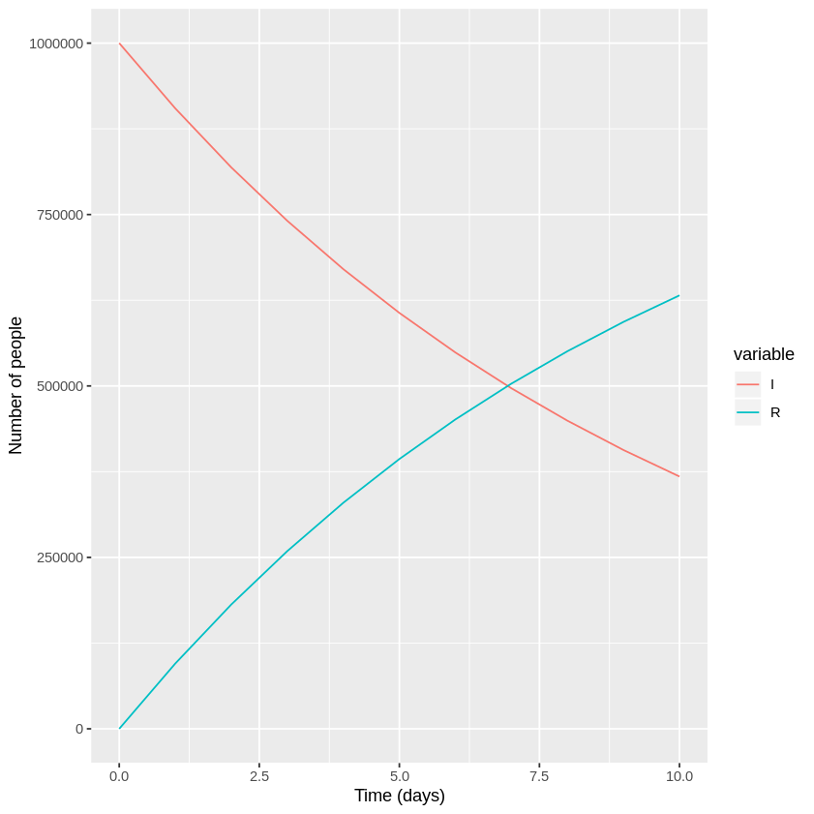
\includegraphics[width=0.8\textwidth]{si-model}
	\caption{Simulation of SI Model}
	\label{fig:si-model}
\end{figure}

\subparagraph{SIR Model}
SIR model is the most fundamental and basic infectious disease model by introducing another compartment called S, which stands for the susceptible compartment.
\begin{align}
	\frac{dS}{dt} & = - \lambda S          \\
	\frac{dI}{dt} & = \lambda S - \gamma I \\
	\frac{dR}{dt} & = \gamma I
\end{align}
$\lambda$ -  \gls{foi}


\begin{figure}[htpb]
	\centering
	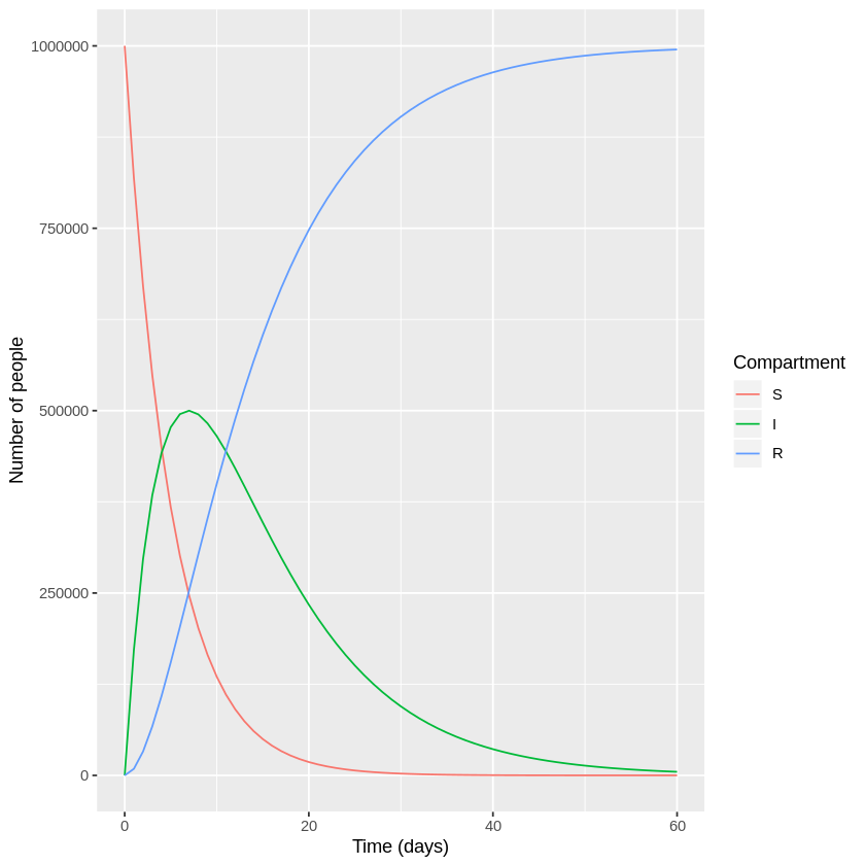
\includegraphics[width=0.8\textwidth]{sir-model}
	\caption{Simulation of SIR Model}
	\label{fig:sir-model}
\end{figure}
\[
	\frac{dS}{dt}=-\lambda S-\mu S+bN
	.\]

The dynamics of an epidemic, for example, the flu, are often much faster than the dynamics of birth and death, therefore, birth and death are often omitted in simple compartmental models.

In the above setting, $\lambda$ or  \gls{foi} is considered as constant. But this does not abide by real world scenario, in which the \gls{foi} will drop down as the susceptible population runs out.
In this setting, the $\lambda$ in SIR model was further extended to be dynamic.
\begin{equation}
	\lambda = \beta \frac{I}{N}
\end{equation}

$\beta$ is the infection rate, and $N$ is the total population.
Different combination of $\beta$ and $\gamma$ was explored by studies, and the ratio between these two key parameters forms the very first idea of \gls{R0}.
\begin{equation}
	R_0 = \frac{\beta}{\gamma}
\end{equation}
\begin{figure}[htpb]
	\centering
	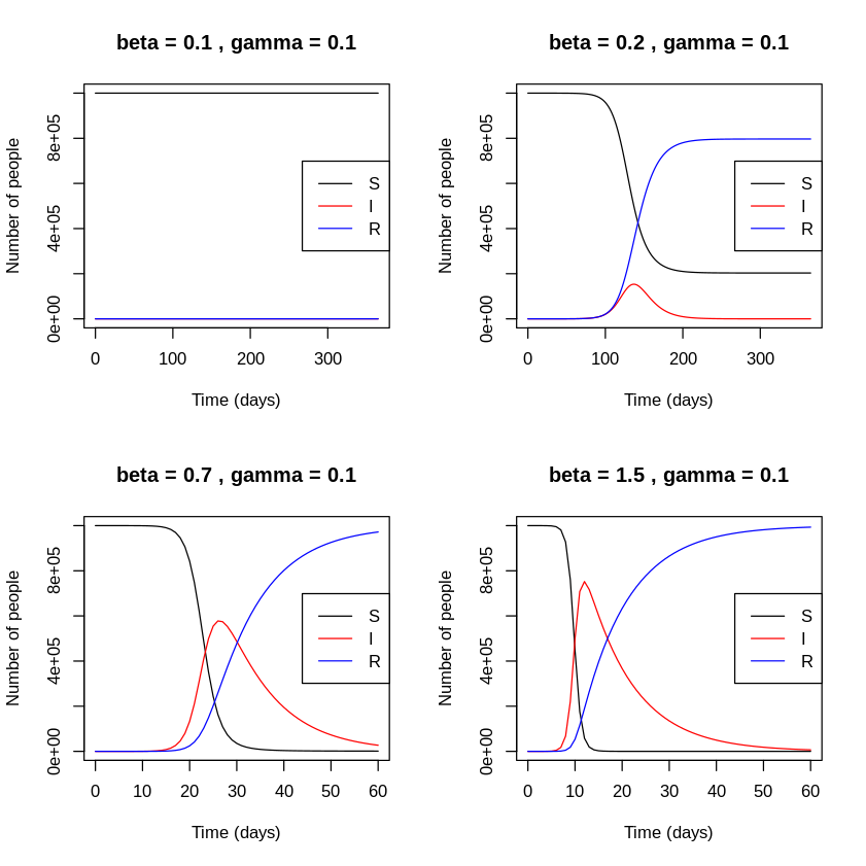
\includegraphics[width=0.8\textwidth]{sir-model-beta-gamma}
	\caption{Comparison of combination of $\beta$ and $\gamma$}
	\label{fig:sir-model-beta-gamma}
\end{figure}

By the definition, if $\beta > \gamma$ the epidemic will take off, and vice versa.
However, the definition of \gls{R0} changes accordingly with the different model.
For example, if the SIR model separate infection group into symptomatic and asymptomatic infection.
\begin{figure}[htpb]
	\centering
	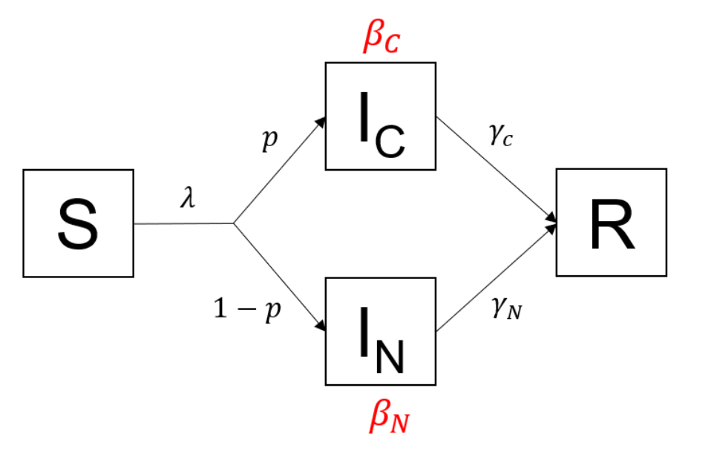
\includegraphics[width=0.8\textwidth]{sir-model-asymptomatic}
	\caption{SIR model structure with asymptomatic compartment}
	\label{fig:sir_model_structure_with_asymptomatic_compartment}
\end{figure}

The calculation of \gls{R0} will change to:
\begin{equation}
	R_0 = p \frac{\beta_c}{\gamma_c} + (1-p) \frac{\beta_N}{\gamma_N}
\end{equation}

Studies further extend SIR model to model population turnover and waning immunity against some disease.
For example, by incorporating birth and death effect in the model, the number of infected people oscillates over time.
\begin{align}
	\frac{dS}{dt} & = - \lambda S - \mu S + bN     \\
	\frac{dI}{dt} & = \lambda S - \gamma I - \mu I \\
	\frac{dR}{dt} & = \gamma I - \mu R
\end{align}
\begin{center}
	$\mu$ - the mortality rate of each group and \\
	$b$ - the birth rate of total population
\end{center}


\begin{figure}[htpb]
	\centering
	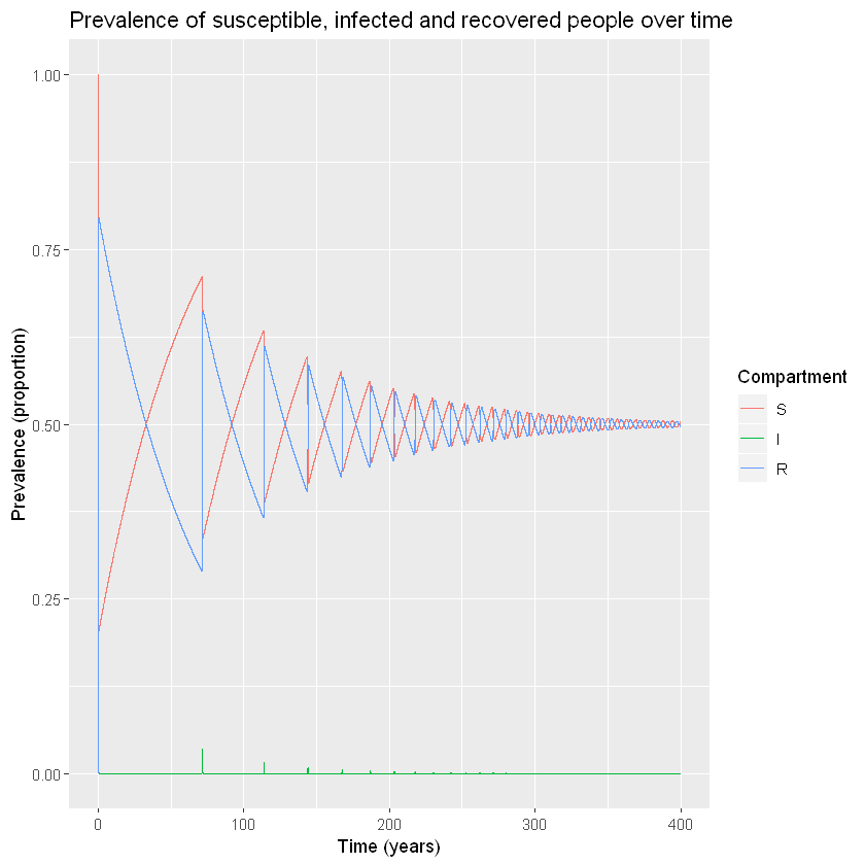
\includegraphics[width=0.8\textwidth]{sir-model-birth-death}
	\caption{SIR Model Simulation with birth and death}
	\label{fig:sir-model-birth-death}
\end{figure}

These are sharp epidemic cycles: epidemics reoccur repeatedly over time, although the peaks become progressively smaller and eventually disappear.
The first peak is the one we looked at above.
This pattern occurs because the disease has a much shorter duration than the human population turnover.
Once an epidemic has spread through the population and depleted the susceptible pool, it takes a long time for the susceptible to replenish through births.
This is why we see these deep and long troughs (around 70 years until the second epidemic) between epidemics.

\paragraph{SEIR Model}
When a pathogen appears in a host community, it partitions individuals in the community into categories depending on parasite density inside them and the type of infection.
These categories or compartments are represented by standard notation of S-E-I-R.
In a simple form they are as follows: the first group consists of the fraction of host population that is Susceptible (S) to infection; then comes the Exposed (E) class - the fraction of population whose individuals are infected by the pathogen, but not capable of passing on the infection to others during a latent period.
The next is I class or Infectious individuals, who give rise to more infected individuals through interaction with the S group.
Finally, those individuals who remove from the infection(mortality or recovered) make up the R class.
There are variations in the compartment structure depending on the type of disease.
For example, the I class of individuals may not recover at all and die; R can consist of individuals, who recover with temporary or permanent immunity, thereby further subdividing the epidemiological compartments.

\paragraph{\gls{vbd} Model}
Ross-McDonald model is the most important 

\begin{figure}[htpb]
  \centering
  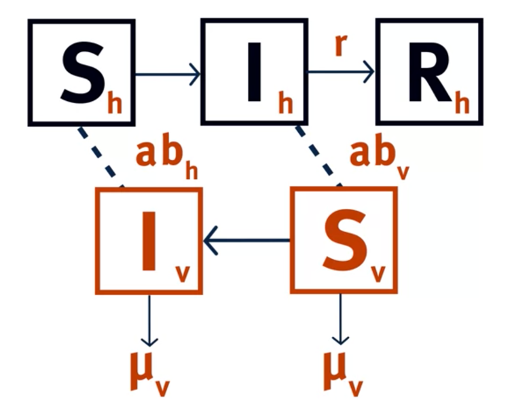
\includegraphics[width=0.8\textwidth]{ross-mcdonald}
  \caption{Ross-McDonald Model Structure}
  \label{fig:ross-mcdonald}
\end{figure}

\begin{align}
  \frac{{dS}_v}{dt} & = \mu_v N_v - ab_vS_v\frac{I_h}{N_h} - \mu_v S_v \\
  \frac{{dI}_v}{dt} & =\ ab_vS_v\frac{I_h}{N_h}-\mu_v I_v \\
  \frac{{dS}_h}{dt} & =\ -\frac{ab_h}{N_h}S_hI_v \\
  \frac{{dI}_h}{dt} & =\ \frac{ab_h}{N_h}S_hI_v-{\rm rI}_h \\
  \frac{{dR}_h}{dt} & =\ {\rm rI}_h 
\end{align}
\begin{centering}
$S_v$ - Susceptible Vector  \\
$I_v$ - Infected Vector\\
$S_h$ - Susceptible Host\\
$I_h$ - infected\ host\\
$R_h$ – recovered host\\
$\alpha$ - biting rate \\
$b_v$ – Probability of infection from an infected host to a susceptible vector\\
$b_h$ – Probability of infection from an infected vector to a susceptible host
\end{centering}

\paragraph{\texorpdfstring{\gls{R0}}{R0}}%
\label{par:R0}
\gls{R0}, the basic reproductive number, is often used as a measure of the severity of disease transmission and the possibility of disease elimination.
Each model could have their own definition of \gls{R0}.
\gls{R0} could be defined as a quantitative answer to the question, “How many infectious humans could be expected from a single infectious human after just one generation of the parasite, assuming all other humans and mosquitoes are susceptible? ”

\paragraph{Interpretation of Vectorial Capacity Equation}%
\label{par:interpretation_of_vectorial_capacity_equation}

One index of malaria transmission intensity is vectorial capacity, the number of secondary cases arising per day from a single infective case in a totally susceptible human population.

Vectorial Capacity is defined by the following equation:
\begin{equation}
 V\ =\ \frac{ma^2p^n}{-\ln{\left(p\right)}} 
\end{equation}

\begin{centering}
$m$ – ratio vector to human\\
$a$ – vector human biting rates\\
$p$	– probability mosquito survive throughout one day\\
$n$	–	\gls{eip}
\end{centering}

Vectorial capacity was analyzed by multiple studies\cite{LeMenach2007a,Bomblies2009b,Briet2019,AnjuViswan2019,Molineaux1978,Gerardin2017,Bomblies2014,Weaver2010a}.
It is closely related to \gls{eir} and \gls{R0}.

\subsubsection{Deterministic vs Stochastic}
\label{subsubsec:deterministic_vs_stochastic}

Malaria mathematical models are generally classified as deterministic or stochastic.
Both deterministic model and stochastic models utilized the concept of compartmental modeling implementation.
Both paradigms of models are useful and have their place in our understanding of malaria and in planning for malaria control.

Other forecasting approaches, including statistical modeling, and machine-learning methods are also being applied in this field.
The statistical methods included generalized linear models, Auto-Regressive Integrated Moving Average (ARIMA) models\cite{box2015time,Anokye2018}, and Holt-Winters models\cite{Chatfield1978}.
Other authors\cite{Toh2021a,Libbrecht2015,Nkiruka2021,Verma2020,Kim2019,Khameneh2014,Ebhuoma2018,Hancock2020} predicted malaria incidence using neural networks, a machine-learning technique.

\paragraph{Deterministic Model}%
\label{par:deterministic_model}

Deterministic models assume the system follows predefined and stationary rules with no random variation or noise and known average rates with no random deviations are applied to large populations.
For example if 1,000 individuals each have a 90\% chance of surviving 1 year, then the deterministic model reasonably assume that 900 of them will indeed survive.

This paradigms assume the randomness is neglectable and combine the average behavior of the system and consider this behavior as a holism perspective.
For the high or intermediate transmission settings, plus systems that do not need to explore heterogeneities, deterministic is a reasonably choice. 
Traditionally, since the scale of malaria incidence was quite large globally, most malaria mathematical models tended to be population-based, treating all individuals with compartment.
Within each compartment, individual were treated as identical.

\subparagraph{When the model is suitable for deterministic model?}%
\label{par:when_the_model_is_suitable_for_deterministic_model_}
Firstly, the less importance of stochasticity in median or high-transmission settings, requires an alternative approach to stochastic compartmental methods.
Secondly, do not require discrete population simulations to incorporate spatially explicit environments at fine resolutions.
Thirdly, do not require to represent heterogeneities in disease progression and severity on the individual patient level.

\paragraph{Stochastic Model}
\label{par:stochastic_model}
Stochastic models assume randomness or noise which is ambiguous or could not be implemented is important and explicitly include it in the system.
Thus, stochastic models explicitly encompass these variates in the architecture.
Detailed stochastic models can provide quantitative evaluations and predictions of the effects of interventions on the levels of malaria transmission, morbidity, and mortality, though they do not always give general rules.
To understand rare events, including malaria death or in elimination settings, a stochastic model is essential.

\subparagraph{\gls{abm}}
\gls{abm} is a class of computational models to simulate actions and interactions between individual based `agents'.
Epidemiological \gls{abm} is a special use case of a broader class of stochastic model.
Multiple simulations are essential for generating meaningful ideas.
The first version of \gls{abm} can be track back to 1971\cite{Schelling1971}.
More recently \gls{abm} have been used to inform public health interventions against flu\cite{Ferguson2006a, Ferguson2005} and COVID-19\cite{Maziarz2020, Ferguson2020, Chang2020}

Modelers are increasingly adopting agent-based approaches, which model hosts, vectors and/or their interactions on an individual level.
One reason for the increasing popularity of such models is their potential to provide enhanced realism by allowing system-level behaviors to emerge as a consequence of accumulated individual-level interactions, as occurs in real populations.

The major advantage of \gls{abm} is the heterogeneity and stochasticity they could provide, but come at the sacrifice of the much higher computational resources.

\subsection{State Transition}
Whether compartmental deterministic or stochastic model, each chamber of model connects to one or many other chambers.
The speed of transition between states are crucial for the models and define the fundamental behavior of different models.
Suppose two compartments at time $t$ in the model called $X_i(t)$ and $X_j(t)$. And the  $i$ to  $j$ transition rate  $p_{ij}$ is the rate of individuals in $X_i(t)$ will move to $X_j(t)$ in the next time step.

For deterministic model, the count of individuals in $X_i(t)$ will decrease because of the flow-out to $X_j(t)$.
Thus, the count of individuals at next time step $t+1$ in $X_i$ is:
\begin{equation}
  X_i(t+1) = X_i(t) - X_i(t)p_{ij}
\end{equation}

For the compartmental stochastic model, three broad methods of individual simulation were commonplace in literatures, each with differing degrees of agent autonomy.

First, models inherited features from compartmental models typically used probabilities in place of flow rates to determine whether an individual transitioned to a new state at a given time step.
Results from a Bernoulli trial dictated state transition.
\begin{equation}
	f(k;p) = p^k ( 1 - p )^{1 - k}
\end{equation}
Where $p$ is the probability and  $k$ is the parameter deciding the rate of transition.

Secondly, some particular models focused on host parasite densities.
Temporal disease state changes governed by a set of equations.

In the third method, specific actions of individuals, for example blood meal searching, resting and oviposition, were simulated according to a process represented by a sequence state chart.

\subsection{Fitting to Real World Data}
Models will only be trusted if they conform to the real world data.
%Maximum likelihood estimation
%Full posterior inference
%\subsubsection{Bayesian Models}
%\subsubsection{MCMC}
Approaches techniques such as \gls{mcmc} \cite{Hastings1970} and approximate Bayesian computation are increasing in popularity as including uncertainty in model parameters becomes more common. 

\gls{mcmc} can search the entire parameter space or part of parameter space that has non-negligible posterior probability and produces a given number of samples.
Results called \gls{mcmc} chain was produced from the parameter distribution. 
The main extension compared to traditional least squares parameter estimation producing one ’best fitting’ point estimate is that \gls{mcmc} create a parameter combination that fit the measured data within the limits of the confidence intervals estimated for the measurements.
\gls{mcmc} has already been used in malaria ensemble modeling\cite{Cameron2015,Penny2015,Penny2015a} and parameter estimation, as well as in modeling of other infectious diseases.
Other variation like reversible jump \gls{mcmc}, which is initialized with a model containing a sub- set of the possible covariates, is also applied in detecting risk factors for malaria transmission\cite{Millar2018a}.

\paragraph{Burn in}%
\label{par:burn_in}
is a widely used method in \gls{mcmc}. The first $n$ iteration in the fitting will be discarded to improve the accuracy.

\paragraph{Uncertainty estimation}
Given that uncertainty remains even after calibration, it is important to apply a systematic and comprehensive approach to parameter estimation before using models for predicting parameter impact or forecasting.

\paragraph{Equilibrium point}%
\label{par:equilibrium_point}
An equilibrium is the simplest possible solution to a dynamical system.
It is a solution where the state variable is a constant; the variable doesn't change with time at all.
Dynamic systems with constant parameters will enter an equilibrium state after a length of simulation.
Studies\cite{Handari2020, Nwankwo2019,NiazArifin2013,Heesterbeek2015a,Karl2016,Olaniyi2020,Stuckey2014,Tompkins2013,Tompkins2013,Mbogo2018,Winskill2019,Smith2019,Briet2013} used the equilibrium state to calculate the parameters, and to explore the optimal interventions coverage of \gls{llins}.

Some studies further altered the intervention parameters to obtain equilibrium states in varying control strategies.
Analysis of the equilibrium points with their local stability and sensitivity analysis of the basic reproduction number \gls{R0} was studied analytically and numerically.
Two types of equilibrium points were analyzed, namely the disease-free equilibrium points and the endemic equilibrium points.
Through other extension method like Pontryagin’s maximum principle, study was able to use numerical simulations to determine an optimal control strategy\cite{Tchoumi2020}.

\subsection{Prediction}%
\label{sub:prediction}

\subsubsection{Choice on the Length of Model Simulation}
3-4 years of length is a common length for simulating the effectiveness of \gls{llins}. However, longer length like 20 years was used in some studies to understand longer term effectiveness\cite{Walker2016}.
\improvement{TODO: an overview of length of model simulation}

\paragraph{time step}%
\label{par:time_step}
Dynamic models may treat time as discrete units, leading to difference equations, or they may consider continuous time, leading to differential equations.

There were also considerations relating the method of agent simulation and size of the time step.
Daily time steps were most common.
A temporal resolution of 1-5 days was suffice to remark the changing disease characteristics.
If agent actions were explicitly modeled, much granular time steps are need.
Hourly status updates were most common, some models even tracked vectors as frequency as each second.

\subsubsection{Intervention Optimization}
A number of papers\cite{Tchoumi2020,Smith2008,Cameron2015,Winskill2019} conducted optimization analysis of interventions.
Methods included changing the location, timing or combination of intervention.
Pontryagin’s Maximum Principle\cite{Tchoumi2020} with respect to a time dependent constant is used to derive the necessary conditions for the optimal usage of interventions.
Non-linear optimization methods\cite{Walker2016} was used to examined how optimum packages vary when control measures are deployed and assessed at national, subnational spatial scales.
Study showed that more granular national malaria control program will result a better cost-effectiveness\cite{Walker2016}.

\subsection{Machine learning}%
\label{sub:machine_learning}
\improvement{TODO: definition of machine learning}
Machine learning offers the ability to extract knowledge from data to identify relevant patterns using classification. These patterns aid in medical diagnosis and decision-making.
Machine learning-based model for the classification of malaria incidence using climate variability.
Methods include K-means, \gls{xgboost}, artificial neural networks were relatively new methods have been widely used in malaria mathematical models.
A neural network is a machine-learning method that connects a set of inputs(eg, weather entomology covariates) to outputs (eg, malaria counts).
The connection between inputs and outputs are made via ‘neurons’ and the number of links and corresponding weights are chosen to give the best possible fit to the training data.
Neural networks have been proved to be useful in their capacity to handle non-linear relationships as well as a large number of parameters, and also their ability to detect all possible interactions between predictor variables.
Study\cite{Verma2020} used backpropagation neural network to predict the incidence of malaria by climate data.

\subsection{Model Assumptions}
Models are only as good as they made reasonable assumptions. In malaria mathematical modeling world, several assumptions have been made. The most important ones ranked as follows,

\paragraph{Homogeneous mixing of population}%
\label{par:homogeneous_mixing_of_population}
In the deterministic types of model, individuals in the same state groups are considered as the same, e.g. Susceptible group has an average probability of transit to infectious group. But the assumption is rarely justified.

\paragraph{Seasonality}%
\label{par:seasonality}
Seasonality: perennial or highly seasonal

Prevalence level: high/moderate/low.
However, up to this date, there is no universal standard to define these levels.
It's lack of guidance for the \gls{nmcp} to categorized their situation.

\begin{table}
	\centering
	\begin{tabular}{c S S S}
		\toprule
		studies & {low} & {moderate} & {high} \\
		\midrule
		S       & 10    & 30         & 60     \\
		\bottomrule
	\end{tabular}
	\caption{Categorization used in modeling studies}
\end{table}

\paragraph{Immunity}%
\label{par:immunity}
Study\cite{White2018b} assumed that both primary infections and relapses contribute to the acquisition of immunity.
And each new infection boosts immunity, after each immune boost there is a refractory period of duration during which immunity cannot be further boosted.

\subsection{How to increase clarity in compartmental models}%
\label{sub:incresing_clarity}
Increasing clarity in model reporting would be of great benefit to both the creators of models and their audience.
While many papers included detailed supplementary materials for additional results, project descriptions and calibration, validation, sensitivity analysis and optimization techniques, the intricacies of these techniques often unclear.
To make model descriptions more understandable and complete, thereby making \gls{abm} less subject to criticism for being irreproducible, a protocol called \gls{odd} \cite{Grimm2010} was published in 2006 to standardize the published descriptions of \gls{abm}.
Some models that used it \cite{Zhu2015, Zhu2015a, Watson2017} were simple to understand and appeared easily replicable by external groups.
Further transparency includes sharing of the mathematics and code{Watson2017} of models.
These small steps in documentation would allow for increased verification and validation of models, as well as increasing opportunities for collaboration between modeling groups.

\subsection{Softwares}

\begin{itemize}
	\item ShinyStan
	\item OpenMalaria
	%\item \href{https://github.com/MWhite-InstitutPasteur/Pvivax_IBM}{Pvivax_IBM}
  \item OpenBugs - \gls{mcmc} fitting \cite{Lunn2009}
\end{itemize}

\section{Host}%
\label{sec:Host}

Key simulated human factors in the models included disease states, demography, host immunity.

\subsection{Disease state}
Human infections begin during the mosquito blood meal when sporozoites enter the skin.
As the greatest public health burden is attributable to \textit{P. falciparum}, most mathematical models focused on the simulations of the impact of interventions on one malaria species, with only few attentions paid on \textit{P. vivax} \cite{White2018b} .

\begin{parameter}
	{latent period from infectious bite to detectable parasites}
	Parasites are not obvious in the blood until about 11 days later.
\end{parameter}

A human with a \textit{P. falciparum} infection is not infectious until a fraction of the blood-stage parasites become gametocytes and then mature.

\begin{parameter}
	{Period of a human get an infectious bite to infectious}
	{8-10 days}
\end{parameter}

Infection with \textit{P. falciparum} can lead to a number of different health outcomes, with a general trend towards decreasing pathology following the gradual acquisition of immunity by exposure and age.
However, immunity is partial and hence episodes can occur across all age groups with asymptomatic carriage of parasite common in older children and adults.
Young children are at risk of severe disease, the life-threatening form of malaria, which typically presents as either severe anaemia or cerebral malaria.
There is no single clear definition of severe disease but in general this form of disease requires hospitalisation.
Severe disease may onset very rapidly or can develop as a consequence of untreated clinical disease.
Clinical disease (also referred to as mild or uncomplicated) is characterised by bouts of recurrent fever due to the cyclical burst of parasites during blood-stage infection.
This is most often defined in research studies and trials on the basis of measured fever plus parasite density in the blood over some threshold, although again there is no single standard definition.
The definition of clinical malaria is similar between models but the number of uncomplicated clinical cases that can occur per infection differs.

\begin{figure}[htpb]
	\centering
	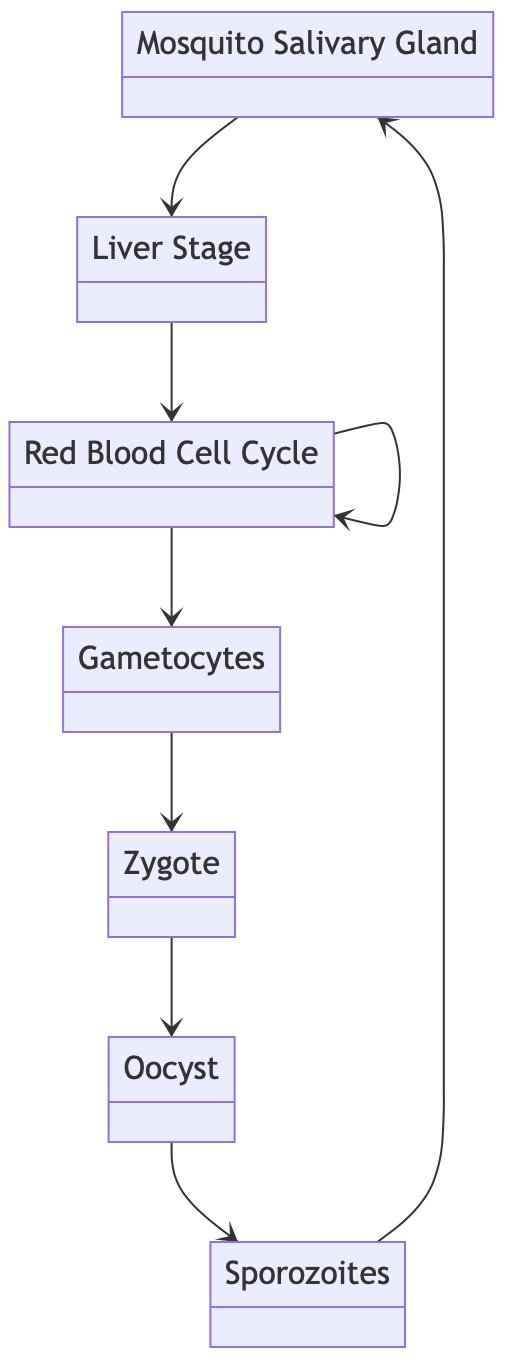
\includegraphics[width=0.2\textwidth]{malaria-life-cycle-diagram}
	\caption{malaria life cycle diagram}
	\label{fig:malaria-life-cycle-diagram}
\end{figure}

\begin{parameter}{\gls{eip}}
	The parasite enters the mosquito during a blood meal and the mosquito becomes infectious 10-16 days later, after the parasite develops into sporozoites.
	The period was called \gls{eip}.
\end{parameter}

An individual malaria infection can last for many months, during which densities of both asexual parasites and gametocytes vary irregularly as consequences mainly of the developmental cycle of the parasite, of host immunity, and of antigenic variation.
Duration of infection in the model followed convolution of exponential distribution or log normal distribution or fixed.

\begin{parameter}
	{The length of disease.}
	{Untreated or improperly treated infection last about 200 days on average, some could last for more than a year.}
\end{parameter}

Human Host could be in one of the following state:
\begin{itemize}
	\item Susceptible
	\item Treating
	\item Disease(with symptom)
	\item Patently Asymptomatic
	\item Sub-patent stage
	\item Prophylactic protection
\end{itemize}

\begin{figure}[t]
	\centering
	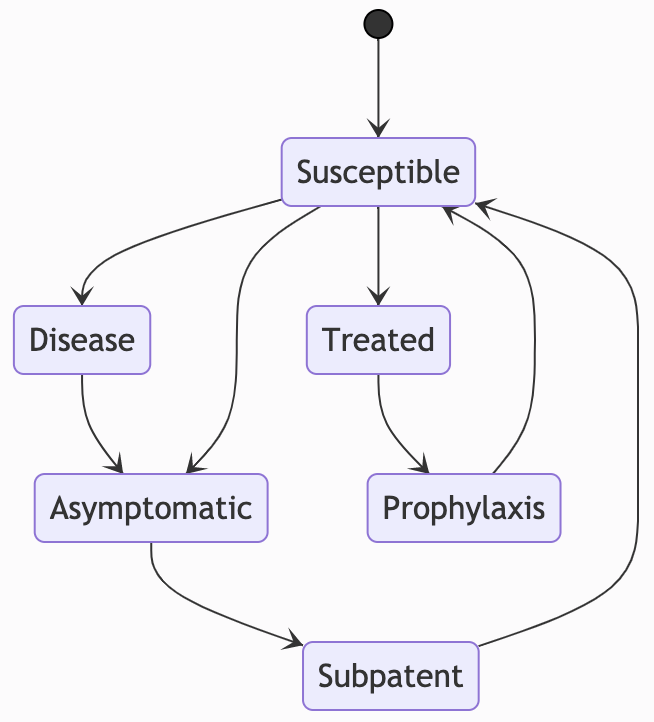
\includegraphics[keepaspectratio=true, scale=0.8]{images/disease-state-transition-diagram.png}
	\caption{Human host disease states transition}
\end{figure}

Models from \gls{swisstph} had at their core individual humans with varying parasite densities. The varying level then will affect the possibilities of the state transition. Infected human will be more likely transit to the next level when they have higher densities.

Models from GSK predicted the clinical malaria based on parasite densities using MAP categories fro low, moderate and high transmission.\cite{Hay2004}

Other study separate infected individuals into three different groups(infected high-density parasites with fever, \gls{pvprlm}, infected PCR detectable parasites)\cite{White2018b}, by symptoms and detectability.

\subsection{Demography}
Demographics of simulated human populations in the models were harmonised with birth cohort and population sizes.
For Imperial the age structure of the population was derived from the life table for Tanzania 2010.
For OpenMalaria a similar distribution was used, although with a higher mortality in the first year of life.
For GSK and EMOD DTK a simple geometric distribution was used that provided a close match to other groups.
In all models the total number of simulated individuals was fixed with a non-growing static population for baseline projections.

\subsubsection{Age}
\improvement{TODO: Of xx papers, xx stratified individuals by age}
Commonly, age was used in the calculation of human biting rates, because of its strong correlation with body surface area.
Other age-varying factors were adaptive and maternal immunity and duration of infection.
\gls{pfpr} was usually calculated at age groups.
If intervention were targeting specific age group, for example \gls{rts}, stratification in model output was used to assess the impact at different age groups.

Relationship between age and incidence was compared between models.

Human population data
Often lack in some areas
Could be estimated through satellite observations
Paper high resolution population maps for low income nations: combining land cover and census in East Africa

\subsubsection{Birth and Death}
Birth and death was simulated in some \gls{abm} models.
Birth was carefully calculated to ensure a constant population in \improvement{TODO: add citation}.
However in south Saharan African countries, the stalled decreasing trend of malaria cases may related to the increasing population.

An universal death rate was introduced to some models \improvement{TODO: add citations} to ensure a constant age distribution. Death rate was also calculated based on the severity of malaria infection.

\subsubsection{In and Out}
Increasing human mobility is creating highly favorable conditions for the persistence of diseases being targeted for elimination.
Host mobility is not a top priority factor for the malaria model.
In malaria elimination scenario, imported cases is an most important threat.
Modeling population flow in that case would be helpful for countries in elimination stage to quantify the threats.
In that case, predictive models of human movement are needed to help inform how best to target strategies.

Only a few models\cite{Zhu2015a} considered the human mobility.
One study focused to fit trip data to the gravity model and radiation model\cite{Marshall2018}.
The relationships between travel distance and frequency was studied.
Other model\cite{acevedo_spatial_2015} used extend Ross-Ronald model to the interplay between spatial transmission heterogeneity and human mobility, and their combined influence on prevalence and \gls{R0}.
These models may help predict the spatial transmission of malaria parasites and inform strategies to control their spread.

On the contrast to host mobility, vector mobility is rarely included in the mathematical models.
Vector mobility may be an important factor especially for the impact analysis of invasive vectors such as \textit{An. stephensi}.

\subsection{Immunity}

Immunity was depicted as being dependent on levels of anti-parasite immunity (AP) and clinical immunity (AC).
In particular, anti-parasite immunity is assumed to have two effects:
\begin{itemize}
	\item reducing the probability that a blood-stage infection will achieve sufficiently high density to be detectable by light microscopy);
	\item increasing the rate at which low density infections are cleared (rPCR).
\end{itemize}
Clinical immunity is assumed to reduce the probability that a high-density blood-stage infection will progress to cause a symptomatic episode of clinical malaria.

The immunity was separated into several categories:

\paragraph{Maternal Immunity}%
\label{par:maternal_immunity}
Children will get the maternal antigen from mother.
Model assumed a new-born infant will acquire a fraction of their mother’s anti-parasite and clinical immunity.
The maternal immunity will protect new born infant from infections, and will decay exponential after a period of time.
\[
	I_{maternal} = e^{- \frac{a}{d_{maternal}}}
	.\]

Here,

\begin{parameter}
	{$I_{maternal}$}
	{denotes maternal immunity.}
\end{parameter}
\begin{parameter}
	{$d_{maternal}$}
	{denotes the exponential decay rate of maternal immunity.}
\end{parameter}
\begin{parameter}
	{$a$}
	{denotes the age.}
\end{parameter}

\paragraph{Acquired immunity}%
\label{par:acquired_immunity}
Acquired immunity.`\ ' including clinical immunity and \improvement{add another type}.
Acquired immunity alters the likelihood that infection results in clinical disease, modifies onward infectivity to mosquitoes, affects the detectability of infection, and modifies the duration of parasitaemia.

\paragraph{Acquisition}%
\label{par:acquisition}
The \gls{abm} explicitly depicted the acquisition of both anti-parasite and clinical immunity to be age and exposure dependent.

\paragraph{decay}%
\label{par:decay}
Specific antibodies against \textit{Plasmodium} decay over time.

\improvement{TODO: among xx studied paper, xx dictated the rate of decay of immunity level}
Different versions of models describe the rate of immunity decay differently.
Exponential decay of naturally acquired immunity was implemented in Imperial models.

\improvement{TODO: Describe the decay rate mathematically}

Immunity level then will be incorporated into models and will affect the probability that an infection becomes detectable, the duration of a blood-stage infection.

\section{Vector}%
\label{sec:vector}
Models most commonly assessed the interventions impacting vector mortality, such \gls{irs}, \gls{itn} and larval source management.
Detailed implementation of vector life cycle and entomology were common.
Mosquito behaviors, such as lifespan, density-dependent larval development, feeding and resting behavior, feeding habits, movement patterns and biting frequency, often modeled in detail.
When models also included a spatial component, malaria transmission generally required vector and host to be co-located.

\subsection{Entomology}
Simulations used a ‘decision tree’ to represent the timing of movements and other necessary actions.
The gonotrophic cycle of a female mosquito begins with a blood meal taken from a host.
The mosquito will rest and wait for digestion.
It may take several blood meals before searching for a breeding site for oviposition.
After egg maturation, the mosquito tries to find a suitable site and then lay 80 – 100 eggs.
Then mosquitoes will search for another blood meal and repeat the gonotrophic cycle.
Larvae emerge from eggs.
After four morphologically larval instars, larvae transform into pupae which develop into adult mosquitoes.
The duration of the larval period depends mainly on temperature, lasts 7-15 days in tropical areas.

\begin{figure}[htpb]
	\centering
	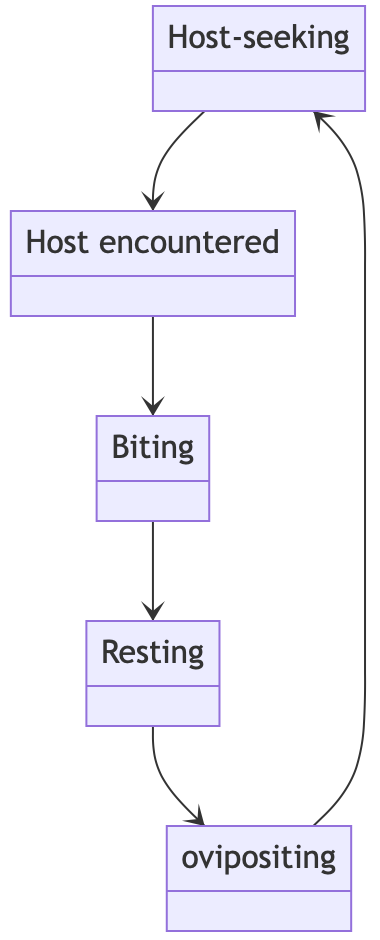
\includegraphics[width=0.2\textwidth]{gonotrophic-cycle-diagram}
	\caption{Gonotrophic cycle diagram}
	\label{fig:gonotrophic-cycle-diagram}
\end{figure}

\subsection{Adult Mosquitoes}

\subsubsection{Species}
\textit{An. gambiae} is the dominated species used in most models.
However different species, including \textit{An. arabiensis}, \textit{An. vagus}, \textit{An. stephensi}, \textit{An. darlingi}, were also included in some other models.
Different combinations of species were also common in the implementation.
The host preferential and feeding habits of different species are the most important factors affect the intervention effectiveness.
Generally, the lower proportion of human blood feeding and night blood feeding, the lower the efficiency of the intervention targeted at protection in night, such as \gls{llins}.

\subsubsection{Endophily}
Research papers often take endophily as a fixed parameter in the model, which means for each different vector there is one according level of endophily.

And the model used in the research often use a

Does endophily change over time or based on the seasons? Often in the cold weather, some vector species tend to reside in the indoor environment. Not covered in the papers.

\improvement{Create a database from research papers to see the different settings of endophily of vector species}

\paragraph{Daily survival rate}

\paragraph{Human visiting rate}

\paragraph{Extrinsic Incubation Period}
Average incubation period in days
Extrinsic incubation period
Features describing a group of vectors (may influenced by interventions)
The composition of the species of given an area
The distribution of vectors
The overall birth rates of vectors
Types of birth rates defined in the papers
fixed (constant)
The distribution of the length of feeding cycle
Related to species, interventions used
\improvement{add two figures(using normal distribution)}
Distribution before intervention
Distribution after intervention

The distribution of the life span of a given group

\paragraph{Cycling Repeating Rate}
Cycling repeating rate

\paragraph{Flying ability}
How long could it fly in a given time

Mathematical function:

A spatial distribution for a given time, e.g.

The ability could determine whether an infectious bite could be transmitted from one to another in a long distance.

\improvement{TODO:
	Add distribution example
	Add mathematical function
	Collect information from papers and create a database}
\paragraph{HBI}
\gls{hbi}
Related to species, intervention
Usage of \gls{llins} and/or \gls{irs} will discourage human biting divert more bites onto non-human hosts

The birth rates may vary in the different settings.
E.g. `\ ' for a colony of germ in the, the reproduction process follows to a logistic growth:
\improvement{TODO: added an example figure of logistic growth}

Does the birth rate of vectors follow the same line?

\subsection{Larval}

Larvae feeds on yeasts, bacteria and organic matters.
After four moults, larvae become pupae, and then develop into adult mosquitoes.

\paragraph{Carrying capacity}%
\label{par:carrying_capacity}
\begin{parameter}
	Carrying capacity, describe how many mosquito larvae or pupae an environment can support.
\end{parameter}

\paragraph{competition}%
\label{par:competition}
Two different forms of density-dependent competition in the larval stages:

\begin{itemize}
	\item contest competition: number of larvae reaches a limit as initial edge density increases. Due to (i) increased mortality at higher density (ii) increased developmental time (iii) reduced larval size.
	\item scramble competition: number of larvae decreases at higher initial egg density. Due to (i) cannibalism of early instar larvae by late instar and (ii)increased population of predators.
\end{itemize}

Environmental larval source management -- reduce carrying capacity

IRS or LLINs - reduction in oviposition -- reduce density-dependent competition between larvae -- decreased larval mortality

\paragraph{Larval Population Dynamics}%
\label{par:larval_population_dynamics}

\begin{parameter}
	\label{para:eggs_laid_per_day}

	Eggs Rate: $\beta$, number of eggs laid per day by each female mosquito.
	\[
		\beta=\frac{eggs\:laid\:in\:life\:time}{expected\:life\:time}
		.\]

\end{parameter}

\subsection{Vector Resistance Against Chemicals}

Discriminating dose bioassays (WHO tube assay, WHO cone assay, CDC bottle assay) are a practical option for control programmes to assess the proportion of the mosquito population that are killed by a standard dose.
Although the simple bioassay has its limitations, it provides a useful measure to link the severity of mosquito insecticide resistance estimated in the field to the results of experimental hut trials evaluating new products.

Strong association between the level of resistance and mosquito mortality observed in the experimental hut trial\cite{Sherrard-Smith2018b}.
\unsure{to understand how they made the connection: did the researcher match the bioassay result to the experimental hut trial data? Find conclusions and methods in the paper and summarized it in this document.}
\unsure{how does mosquito resistance affect the repel rate? Why do the mosquitoes don't like the pyrethroid  smell? And why does the mosquitoes' repel rate drops down when the resistance level goes up?}

Resistance level in discriminating bioassay: the percentage of mosquitoes surviving 24-hours following exposure.

The impact of reduced susceptibility of mosquito:
\begin{itemize}
	\item the initial efficacy is reduced
	\item the active life-length of the insecticide is shorter as fewer mosquitoes are susceptible
\end{itemize}

\change{add the mathematical equation that describe the decrease.}

One comment on the second point is that it seems there are some certain level of threshold for the resistance level and active ingredient. When combining these two factors, we might able to calculate the overall efficacy of the effective length.

An epidemiology-genetics model was published\cite{Mohammed-Awel2019} for assessing the impact of insecticides resistance in the mosquito population.
The model couples disease epidemiology with vector population genetics and studied the equilibrium state of an deterministic dynamic malaria model and presented the resistance allele dominance associated with the insecticide resistance in the mosquito population.
Study showed that in moderate and high malaria transmission settings the \gls{itn}-\gls{irs} strategy can lead to the effective control of the disease, but in longer simulation it fails to manage insecticide resistance (as measured in terms of the frequency of resistant allele).

\subsubsection{Measurement of Resistance}

Bioassay:

\begin{itemize}
	\item Discriminating Bioassay
	\item Intensity Bioassay
	\item Mechanism Bioassay
	\item Non-standard Bioassay
\end{itemize}

\section{Force of Infection and EIR}%
\label{sec:force_of_infection_and_eir}

\subsection{\texorpdfstring{\gls{foi}}{Force of Infection}}%
\label{sub:foi}

\subsection{\texorpdfstring{\gls{eir}}{EIR}}%
\label{sub:eir}
\gls{eir} is the driving parameter of malaria mathematical models.
Three of the models are driven by \gls{eir} (EMOD DTK, Imperial and OpenMalaria).
Only few models use prevalence rather than \gls{eir}as the input.
By varying the corresponding EIR ranged from 0 to 512 infectious bites per person per year, relationship between \gls{eir} and intervention outcomes was studied.

\section{Model Output}%
\label{sec:model_output}

\paragraph{Index}%
\label{par:index}
Model output include:
\begin{itemize}
	\item Clinical cases
	\item All severe cases and hospitalized
	\item Death due to malaria
	\item \gls{dalys}
	\item Cost-effectiveness
\end{itemize}
$PfPR_{2-5}$, $PfPR_{2-10}$\cite{Penny2016}, number of cases averted, \gls{dalys} are the most common indexes.
The prevalence of infection is defined by microscopy(\gls{pvprlm}) and PCR by specified age group.
Comparison between baseline settings and outcome was conducted to understand the effects on interventions.

\subsection{\texorpdfstring{\gls{dalys} calculation}{DALYs Calculation}}%
\label{sub:dalys_calcualtion}
\gls{dalys} were calculated based on the duration of disability and respective disability weights.
Weights by disease outcome and treatment have been obtained from the Global Burden of Disease Life-time disability is assumed for severe episodes that result in neurological sequelae.
Years of life lost (YLLs) and DALYs were calculated assuming age-specific life expectancies, based on the life-table from countries.
YLLs and DALYs were estimated based on a comprehensive measure of deaths that includes both direct malaria deaths and deaths due to malaria co-morbidities.
While some model only focus on mobility based on direct malaria deaths.

\subsection{Cost Effectiveness}%
\label{sub:cost_effectiveness}
\gls{icers} was the main index for comparing cost effectiveness.
For example, \gls{icers} was compared between four models in one study to analysis the cost-effectiveness of \gls{rts} \cite{Hay2004}.

\section{Interventions}
Interventions could broadly be divided into those targeted at the human host (e.g. pharmacological) or the vector.

Two core interventions defined by WHO: \gls{llins}, \gls{irs}

Effects of \gls{llins} and \gls{irs}:

\begin{itemize}
	\item Deferred from entering, measured by by the number of mosquitoes caught in a hut with an intervention compared to a control hut
	\item enter the hut and either exit without feeding
	\item Die
	\item Successfully blood-fed
	\item Lower down the survival rates for adults mosquitoes in \gls{eip}
	\item less eggs being oviposited in breeding sites
\end{itemize}

Effects of \gls{irs} \cite{Sherrard-Smith2018b}:

\gls{irs} product effectiveness varies depending on factors including:

\begin{itemize}
	\item impact on mosquito populations (for example, an ability to kill or deter mosquitoes from entering a sprayed structure);
	\item impact duration (the residual half-life);
	\item where and when sprays are deployed (local malaria endemicity, seasonality of transmission and timing of IRS, mosquito species, human behavior and net-use), and;
	\item spray quality and coverage.
\end{itemize}

Realistic intervention variables, including attrition of LLINs due to wear and tear, waning of insecticides used within IRS or LLINs, and prespecified correlation between interventions and rounds of the same intervention was included in some models\cite{Walker2016}.

Interventions targeting adult mosquitoes have the benefit of reducing the probability that an infected mosquito survives sporogony to become infectious, but reduced oviposition will lower the inner competition of larvae, hence reduce the mortality of larvae.
While, interventions targeting larvae will result in a drop in mosquito density, but the proportion of infected mosquitoes will remain the same, or even increase(due to the reduced competition in adult mosquitoes for blood meals)

\subsection{\texorpdfstring{\gls{llins}}{LLINs}}%
\label{sub:llins}

\paragraph{Interval of simulation}%
\label{par:interval_of_simulation}
Mass campaign was a popular way to distribute \gls{llins} in \gls{ssa}.
Interval between campaigns are crucial for sustain the effectiveness of nets.
A variety of intervals were used in the models.
Among which, 2, 3, 4\cite{Walker2016} were the common choices.

Studies showed the declined trend of \gls{llins} effectiveness due to the attrition of the pyrethroid and integrity of the net.
Overall effectiveness will be less influenced by attrition for a short interval.

\subsection{effectiveness}
\improvement{TODO: what kind of index studies focused? EIR? DALYs? Prevalence?}
Studies focused on the assessment of the impact of interventions on malaria transmission, mosquito prevalence, \gls{eir}, cases averted.

Prevalence results from Uganda \gls{rct}\cite{Staedke2020}:
\begin{center}
	\begin{tabular}{c c c c}
		Type        & 6 months & 12 months & 18 months \\
		\hline
		\gls{llins} & 15       & 13        & 14        \\
		\gls{pbo}   & 11       & 11        & 12        \\
	\end{tabular}
\end{center}

\subsection{attrition}

\paragraph{Half life}%
\label{par:half_life}

A half-life of effectiveness 2.64 years

From Tanzania\cite{Protopopoff2018} \gls{rct}, the permethrin and \gls{pbo} concentration dropped at a steady rate for both standard \gls{llins} and Pyrethroid-PBO \gls{llins}:

\begin{center}
	\begin{tabular}{cccc}
		\toprule
		chemical             & 0 months & 12 months & 21 months \\
		\midrule
		Permethrin (Regular) & 21.4     & 21.5      & 16.7      \\
		Permethrin (PBO)     & 20.9     & 14.7      & 12.2      \\
		PBO                  & 9.5      & 2.9       & 1.6       \\
		\bottomrule
	\end{tabular}
\end{center}

From Uganda\cite{Staedke2020}, the \gls{pbo} dropped:
\begin{center}
	\begin{tabular}{c c c}
		\toprule
		chemical     & 0 months & 12 months \\
		\midrule
		PermaNet 3.0 & 26.18    & 15.28     \\
		Olyset Plus  & 8.17     & 5.04      \\
		\bottomrule
	\end{tabular}
\end{center}

Usage attrition from Tanzania\cite{Protopopoff2018}:

\begin{center}
	\begin{tabular}{c c c}
		\toprule
		index     & 4 months & 21 months \\
		\midrule
		ownership & 97.6     &           \\
		access    & 89.6     & 70.2      \\
		usage     & 76.9     & 50.6      \\
		\bottomrule
	\end{tabular}
\end{center}

\begin{center}
	\begin{tabular}{c c c c}
		\gls{irs}      & 0 months & 9 months & 12 months \\
		Actellic 300CS & 0.99     & 0.82     & 0.59      \\
	\end{tabular}
\end{center}

Usage attrition from Uganda\cite{Staedke2020} showed a much slower trend in the decease in usage:

\begin{center}
	\begin{tabular}{c c c c}
		index             & 6 months & 12 months & 18 months \\
		ownership         & 97       & 95        & 91        \\
		adequate coverage & 71       & 63        & 51        \\
		usage             & 85       & 79        & 73
	\end{tabular}
\end{center}

\subsection{PBO}

\[
	PBO = 3.41 + 5.88 \frac{((1-\beta) - 0.5)}{1 + 0.78 ((1-\beta) - 0.5)}
	.\]
\[
	\gamma_a = \frac{e^{PBO}}{1 + e^{PBO}}
	.\]
\[
	\gamma_a = 1 - \beta
	.\]
\[
	\gamma_h' = 0.63 + 3.997 ( \gamma_a - 0.5 )
	.\]
\[
	\gamma_h = \frac{e_{\gamma_h'}}{1+e^{\gamma_h'}}
	.\]

\subsection{IRS}
Four insecticide gradients, pyrethroids (including deltamethrin, lambda-cyhalothrin and alpha-cypermethrin) are the main insecticides used by \gls{nmcp} for \gls{irs}.

\section{Environments}%
\label{sec:environments}
Core environmental aspects related to vector activity were included, such as water sources for oviposition (egg-laying)\cite{Bomblies2008}, houses for blood meal locations\cite{Gu2009a}, and meteorological data to account for seasonal patterns in transmission\cite{Depinay2004}.
Rainfall and temperature data were regularly used; model questions included the impact of wet season lengths\cite{Endo2016a} and hysteresis\cite{Yamana2017} on vector populations.

Environmental factors such as temperature and rainfall at different times was incorporated in some models.


\section{Costs}
Cost of Interventions increases when coverage increase.\cite{Winskill2017a} considered two approaches to simulate the function:
\begin{itemize}
	\item linear increases in cost associated with increasing coverage
	\item delivery cost increases logarithmically with increasing coverage
\end{itemize}

Total cost was assumed to consist of two components: the commodity and the delivery. The commodity part of cost follows U-shape curves follows the marginal cost formula.

$$ MC = \frac{\Delta C}{\Delta Q} $$

In the short run, marginal cost ($MC$) drops when quantity($Q$) increases, then increase as $Q$ increases.

The delivery part increase as coverage increase. For the linear assumption, J

\begin{table}[htpb]
	\centering
	\caption{Cost of Malaria Interventions}
	\label{tab:cost_of_malaria_interventions}
	{\small
		\begin{tabular}{cSSSSSSSS}
			\toprule
			Studies           & {year} & {distributing \gls{llins}} & {\gls{irs}(per person per year)} & {three rounds of seasonal Chemoprevention(per child per year) } & {Non-drug cost of mass screen and treatment (per person per round)} & {Non-drug cost of mass drug administration (per person per round) } & {Full course of dihydroartemisin-piperaquine} & {Treatment of uncomplicated malaria with artemether-lumefantrine} \\
			\midrule
			\cite{Walker2016} & 2016   & 7.03                       & 8.80                             & 5.25                                                            & 5.63                                                                & 2.98                                                                & 1.65                                          & 2.50                                                              \\
			\bottomrule
		\end{tabular}
	}
\end{table}

\subsection{\texorpdfstring{\gls{llins}}{LLINs}}
Review from fields were used to estimate the median unit procurement cost and the delivering cost of \gls{llins}.
Inflation rate calculator was also included in some studies\cite{Walker2016}.

\begin{table}[htpb]
	\centering
	\caption{Cost of \gls{llins}}
	\label{tab:cost_of_llins}
	\begin{tabular}{cSSSS}
		\toprule
		studies           & {year} & {procurement} & {delivering} & {total} \\
		\midrule
		\cite{Walker2016} & 2016   & 5.00          & 1.58         & 7.03    \\
		\bottomrule
	\end{tabular}
\end{table}

\subsection{\texorpdfstring{\gls{irs}}{IRS}}
Range from USDA 2–3 to roughly USDA 20 per unit\cite{Oxborough2016}
(a unit is standardized across products to cover approximately 250 of wall surface)

\begin{table}[htpb]
	\centering
	\caption{Cost of \gls{irs}}
	\label{tab:cost_of_irs}
	\begin{tabular}{cSSSS}
		\toprule
		studies           & {year} & {procurement} & {delivering} & {total} \\
		\midrule
		\cite{Walker2016} & 2012   &               &              & 8.08    \\
		\bottomrule
	\end{tabular}
\end{table}

Perennial and seasonal settings were two concepts describing the seasonal feature in sub-Saharan region.

\subsection{\texorpdfstring{\gls{rts}}{RTS}}%
\label{sub:rts}
Costs of vaccine introduction are calculated by some studies\cite{Hay2004} from the provider perspective, but are limited to cost of
consumables including vaccines, injection and reconstitution syringes, safety box.
Prices are scaled up to account for freight\cite{Winskill2017a} and wastage\cite{Hutton2006}.

\section{Parameters}
Further, no previous models have calibrated all parameters to data.

\paragraph{Sources}%
\label{par:sources}
The methods for estimating key parameters varied greatly across the literature.
Most models used past literature or simulations to determine baseline parameter values.
Due to the nature of certain inputs, many parameters cannot or have not been estimated in field studies, and consequently authors used expert knowledge to select these values.

\paragraph{Calibration}%
\label{par:calibration}
Parameter justification was not always clear\cite{Gurarie2007,Arifin2011a,NiazArifin2013}; when explained, models generally calibrated a range of parameters to existing data, or provided references for their choice of fixed values.
Studies used models that were either previously calibrated to data or presented calibration as a component of their work.
Calibration techniques included the use of calibration vectors, least squares, maximum likelihood functions, and visual estimations.
Bayesian techniques for model fitting could provide credible intervals alongside point estimates of parameters.
Calibrating all model parameters to data is not implemented by most researchers, which necessarily excludes certain parameter combinations that could produce accurate calibrations.

\paragraph{Equilibrium state}%
\label{par:equilibrium_state}
Model also take the advantage of equilibrium state to estimate the parameters\cite{Alves2021}.
Static models assume the system has reached a steady state solution that does not change with time.
Static models are simpler to formulate and analyse.
Dynamic models study the evolution of a system over time.
Dynamic models can be either deterministic or stochastic, each version could lead to an equilibrium points.
Studies calibrate part of parameter set by assuming the region has reached the equilibrium state.

\begin{parameter}
	{Average eggs lay by female \textit{Anopheles}}
	80 - 100 eggs.
\end{parameter}

\begin{parameter}
	{Duration of the larval period}
	Depends on temperature, in tropical areas, lasts 7 - 15 days.\cite{bayoh_lindsay_2003}
\end{parameter}

\begin{parameter}
	{Carrying capacity in aquatic stage}
	Describe how many mosquito larvae/pupae an environment can support
\end{parameter}

\subsection{Experimental Hut Trail}
Experimental hut studies typically report 24-h productinduced: mortality, blood-feeding inhibition, exophily and deterrence.

Outcome:

\begin{parameter}
	\label{eht:mortality}

	Mortality: The number of female mosquitoes found in the hut which are dead on collection or die within the next 24-h
	\[
		Mortality = \frac{D}{N}
		.\]
\end{parameter}


\begin{parameter}
	\label{eht:exophily}

	Exophily: the number of female mosquitoes in exit traps (E) compared to the sum of the number collected in the hut and exit traps (N)
	\[
		Exophily = \frac{E}{N}
		.\]

\end{parameter}

\begin{parameter}
	\label{eht:blood_fed}

	Blood feeding: The number of mosquitoes that are blood fed which were collected in the hut and exit traps
	\[
		BloodFed = \frac{B}{N}
		.\]
\end{parameter}

\begin{parameter}
	\label{eht:Deterrence}

	Deterrence: Reduction in the entry rate of mosquitoes into experimental huts with or without.
	\[
		Deterrency = \frac{N_C - N_T}{N_C}
		.\]
\end{parameter}

Explanatory factors:

\begin{parameter}
	\label{eht:experimental_hut_types}
	Experimental hut types: West or East African design

\end{parameter}

\begin{parameter}
	\label{eht:wall_substrate} Wall substrate: Cement or mud

\end{parameter}

\begin{parameter}
	\label{eht:chemical_class_used}
	Chemical types used in \gls{eht}.

	For IRS: carbamate, clothianidin, organophosphate and pyrethroid

	For LLINs:
	\improvement{TODO: list the chemical class used in the LLINs}

\end{parameter}

Prediction of \gls{eht} outcomes using explanatory factors, combining linear algebra and non-linear transformation\cite{Sherrard-Smith2018b}:

\[
	\pi_i = logit^{-1} \frac{\ln \pi_i}{1-\pi_i} = \frac{ \exp( \beta + \sum_h \beta_h X^{hi} ) }{ 1 - \exp( \beta + \sum_h \beta_h X^{hi} ) }
	.\]

$\beta_h X^{hi}$ denotes explanatory factors times covarite, which is the linear transformation of the explanatory hypothetical space. The middle part of the formulation then project $\mathbb{R} \twoheadrightarrow (0,1)$.

\section{Evaluation and Validation}
Accurate predictions of malaria can provide public health and clinical health services with the information needed to strategically implement prevention and control measures.
Many \gls{abm} had an emphasis on informing policy and explicitly aimed to understand specific programmatic questions.
To reliably inform public health decisions, there must be confidence in the assumptions guiding model creation, in particular regarding choice of parameter values.
If modeling groups are considering extending their model frameworks, particularly to influence policy, evaluation and validation against real-world data is necessary.

\subsection{Validation}%
\label{par:validation}
Validation was performed on some models.
All major model frameworks were reported as validated.
Validation techniques were rarely explained in detail.
When described, validation was most commonly performed by running a calibrated simulation, and comparing model outputs to a dataset not used for calibration.
Methods like root mean squared error and absolute difference\cite{Adimi2010, Rahman2011}, 95\% CI(for predicted value and compared to observed)\cite{Chatterjee2009,Gomez-Elipe2007,Roy2011}, average percentage error\cite{Haghdoost2008}, T-test\cite{Xiao2010}, coefficient correlation\cite{Yacob1947} were used.
For example, validation against \gls{rct}, or \gls{eht}.
A typical approach for dealing with data for validation was to segment data into a model building or training portion with one other portion(the 'holdout' sample) used for model validation or assessing forecast accuracy.
Studies\cite{Parveen2021,Rahman2011} implemented these methods to perform model validation.
The studies divided raw data into training and testing groups by excluding the last year of data, then fit to the remaining data.
The accuracy of the predictions was then estimated from the prediction residuals.
In machine learning studies, to prevent over fitting, data were separated into three groups rather than two groups, the training group, cross-validation group and the testing group.
Model will fit the parameters using training group, adjust them by comparing metrics against cross-validation group and validate the final model performance by the testing group.
A number of studies concluded that their model did not accurately fit the data used for validation, suggesting incomplete data may explain any discrepancies.

\subsection{Model Comparison}%
\label{par:comparing_models}
Methods of comparing models to data were rarely explained; use of a square distance function, log likelihoods and docking techniques were outlined.
Successful model validation was often used to justify extending a model framework to include interventions or to assess their potential impact in the location of interest.
Direct comparison of methods would be easier if multiple malaria forecasting methods were applied to the same data.
It would be helpful if we develop a standard dataset and standard index for model comparison.

\begin{table}[htpb]
	\centering
	\caption{Model Heterogeneity Comparison}
	\label{tab:model_heterogeneity_comparison}
	\begin{tabular}{cc}
		\toprule
		model             & \\
		\midrule
		\cite{White2018b} & \\
		\bottomrule
	\end{tabular}
\end{table}

\subsection{Sensitivity analysis}%
\label{par:sensitivity_analysis}
Some studies\cite{Mohammed-Awel2019, White2018b} explicitly mentioned sensitivity analysis or described parameter variation and comparison of outputs.
The techniques used were generally informal, with methods used rarely explained in detail, and reporting of results was uncommon.
Where sensitivity analysis was explained, it involved altering calibrated baseline parameter values by a fixed percentage and assessing changes to the response function.
Speed of loss rate of \gls{llins} adherence\cite{White2018b}\ldots was studies by the sensitivity analysis.
Formal techniques employed included Latin Hypercube sampling, regression tree analysis, and one-way and probabilistic sensitivity analysis.

\begin{figure}[htpb]
  \centering
  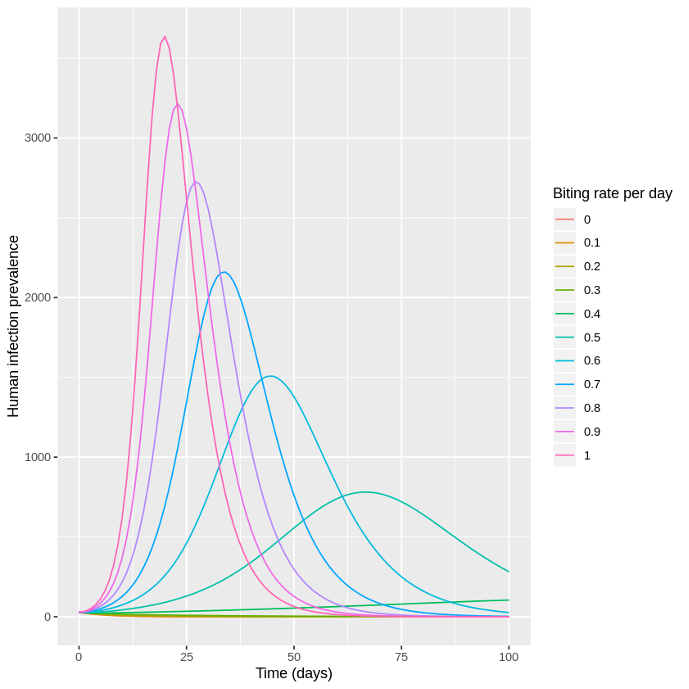
\includegraphics[width=\textwidth]{ross-mcdonald-sensitivity}
  \caption{An example of Sensitivity Analysis with Ross-McDonald Model}
  \label{fig:ross-mcdonald-sensitivity}
\end{figure}

\subsection{Performance metrics}%
\label{par:performance_metrics}
The diversity in forecasting accuracy measures and the use of scale-dependent measures limits the comparability of forecasting results, making it difficult to identify the optimal predictors and methods for malaria forecasting.
Methods like Akaike’s information criterion, Bayesian information criterion, the coefficient of determination, mean absolute error for regression models; classification accuracy, \gls{auc}, F1 score for classification models were used to choose a best fit model parameters.
%to identify and assess methods, including predictors, used to forecast malaria is important for 
\subsubsection{Classification metric}
\paragraph{Classification accuracy}%
\label{par:classification_accuracy}
This is the ratio of the total number of accurate predictions to the total number of input sample used.
\[
	Accuracy = \frac{Accurate predictions}{Total Predictions}
	.\]

\paragraph{\gls{auc}}%
\label{par:auc}
\gls{auc} is used for evaluating binary classification problems.
\gls{auc} score provides a good summary of the performance of the receiver operator curves.
The Receiver Operating Characteristics(ROC) curve was plotted between the false-positive rate (FPR) and true-positive rate (TPR), representing the model’s performance, and then the \gls{auc} score was calculated.

\paragraph{F1 score}%
\label{par:f1_score}

\paragraph{Akaike's information criterion}%
\label{par:akaike_s_information_criterion}

\paragraph{Least-squares estimation}%
\label{par:least_squares_estimation}
R code for least squares estimation calculation:
\begin{minted}
{R}
SIR_SSQ <- function(parameters, dat) {  
    result <- as.data.frame(ode(  y = initial_state_values # named vector 
                            , times = times                # vector of times
                            ,  func = SIR_fn               # SIR function
                            , parms = parameters)
    )

    # assumes the data you are fitting to has a column "I"
    dat <- na.omit(dat) # within the function, 
                        #select complete cases only from dat

    #select from result$I where the times match the times in the data  
    deltas2 <- (result$I[result$time %in% dat$time] - dat$I)^2   
    SSQ   <- sum(deltas2)
    return(SSQ)
    }
\end{minted}

\subsection{Comparing to Randomized Control Trails}

\gls{rct} is the gold standard for assessing intervention efficacy and effectiveness in the field.
Results from \gls{rct} were compared to the model predictions by modellers to determine whether parametrisations satisfactorily match the observed red data\cite{Sherrard-Smith2018b}.
Mean, as well as maximum and minimum impact can be generated by models for assessing.
The parameter sets could be fitted to different \gls{eht} and then compare the results from \gls{eht}.

\subsection{Cross Comparing}
\subsection{Predict Future Results}

\section{Method}%
\label{sec:method}
\subsection{Search strategy and selection criteria}
A literature review was performed.
Database searches of Google Scholar were performed.
Terms relating to malaria, mathematical model, epidemiology, demography, agent-based, individual-based, microsimulation models were included. No limits were placed on publication type, language, location, dates or publication status.

\section{results}%
\label{sec:results}
The search yielded 212 abstracts potentially meeting the inclusion criteria.

\begin{table}
	\centering
	\label{tab:overview_of_the_review}
	\begin{tabular}{c S}
		\toprule
		type             & {number} \\
		\midrule
		inclusion        & 212      \\
		full-text review & 50       \\
		\bottomrule
	\end{tabular}
	\caption{Overview of the review}
\end{table}

% appendix
\appendix
\printglossaries
\printnomenclature
\bibliographystyle{unsrt}
\bibliography{library}

\end{document}
